%%*****************************************************************************
%% $Id: extex-developers.tex,v 1.2 2005/08/29 07:08:02 gene Exp $
%%*****************************************************************************
%% Author: Gerd Neugebauer
%%-----------------------------------------------------------------------------
\documentclass{extex-doc}

\usepackage{subfigure}

\def\setVersion$#1: #2.#3 ${\gdef\Version{#2.#3}}
\setVersion$Revision: 1.2 $

\newcommand\menu{\textsf}
\newcommand\sub{\(\rightarrow\) }
\newcommand\File[1]{\texttt{#1}}

\newcommand\Macro[1]{\texttt{\char`\\ #1}}

\begin{document}%%%%%%%%%%%%%%%%%%%%%%%%%%%%%%%%%%%%%%%%%%%%%%%%%%%%%%%%%%%%%%%

\begin{titlepage}
  \parindent=0pt
  \begin{center}
  \vspace*{1pt}
  \vfill
  \ExTeXbox
  \vfill
  \textsf{\bfseries\Huge Developer's Guide}
  \vfill
  \textsf{\Large Version \Version}
  \vfill
  \textsf{\large Gerd Neugebauer}
  \vfill
  \vfill
%\maketitle

  \begin{abstract}\parindent=0pt
    This document describes some basic steps to develop and test
    \ExTeX.  It is meant for newcomers to the project or people who
    want to evaluate \ExTeX\ by inspecting the sources.
  \end{abstract}
  \end{center}
\newpage
\footnotesize
\copyright\ 2005 The \ExTeX\ Group and individual authors listed below 
\medskip

Permission is granted to copy, distribute and/or modify this document
under the terms of the GNU Free Documentation License, Version 1.2 or
any later version published by the Free Software Foundation. A copy of
the license is included in the section entitled ``GNU Free
Documentation License''.
\bigskip

This product includes software developed by the Apache Software
Foundation (http://www.apache.org/).

\vfill

Gerd Neugebauer\\
Im Lerchelsb\"ohl 5\\
64521 Gro\ss-Gerau (Germany)
\smallskip

\href{mailto://gene@gerd-neugebauer.de}{gene@gerd-neugebauer.de}

\end{titlepage}

\tableofcontents
\newpage

%------------------------------------------------------------------------------
\chapter{Introduction}
%@author Gerd Neugebauer

\ExTeX{} aims at providing a high-quality typesetting system. The
development of \ExTeX\ has been inspired by the experiences with \TeX.
The focus lies on an open design and a high degree of configurability.
Thus \ExTeX\ should be a good base for further development.

On the other hand we have to take care not to leave the current user
base of \TeX\ behind. pdf\TeX\ has taught us that a migration path
from \TeX\index{TeX@\TeX} has a positive value in it. In the mean time
the majority of \TeX\ users applies in fact
pdf\TeX\index{pdfTeX@pdf\TeX}.

To provide a backward compatibility of \ExTeX\ with
\TeX\index{TeX@\TeX} one special configuration is provided. Thus
backward compatibility is just a matter of configuration.


\section{Audience}

This document is meant for developers and those interested in the
sources and development processes of \ExTeX. It should contain all
information for getting started quickly.


\section{Mailing Lists}

If you are ready to try \ExTeX{} you might as well want to join a
mailing list to get in contact with the community. The following
mailing lists might be of interest:

\begin{description}
\item[extex@dante.de] \ \\
  A general mailing list about \ExTeX. It has low traffic and is
  mainly in German. Subscribe and unsubscribe via the Web form
  \url{http://www.dante.de/listman/extex}.
\item[extex-eng@dante.de] \ \\
  A general mailing list about \ExTeX. It has currently very low
  traffic and is in English. Subscribe and unsubscribe via the Web
  form \url{http://www.dante.de/listman/extex-eng}.
\item[extex-devel@dante.de] \ \\
  A mailing list for the exchange of the developers of \ExTeX. It has
  low traffic and is partly in German. Subscribe and unsubscribe via
  the Web form \url{http://www.dante.de/listman/extex-devel}.
\end{description}


\section{Language}

The official project language for \ExTeX\ is English in the US
dialect. The sources are documented in this language and the major
documents are written in this language.

Since some of the developers are German this language might slip in
during intensive discussions.

\section{The Repository}

The sources of \ExTeX\ are stored in a RCS repository. To access this
repository you need access to the internet and RCS installed in some
way.

The coordinates of the repository are:\medskip

\begin{tabular}{ll}\toprule
  Connection type: & \texttt{pserver}			\\
  User:		   & \texttt{anonymous}			\\
  Host:		   & \texttt{cvs.extex.berlios.de}	\\
  Location:	   & \texttt{/cvsroot/extex}		\\
  Module:	   & \texttt{ExTeX}			\\\bottomrule
\end{tabular}\medskip

These coordinates allow you anonymous access to the sources with
reading permissions only.

\section{User Account at Berlios}

To commit changes to the repository you have to be enlisted as a
developer for \ExTeX. A first requirement for this is an account at
Berlios -- the hosting site. 



%------------------------------------------------------------------------------
\chapter{Prerequisites}
%@author Gerd Neugebauer

\section{Java}

You need to have Java 1.4.2 or later installed on your system. You can
get Java for a several systems directly from \url{http://java.sun.com}.
Download and install it according to the installation instructions for
your environment.

Free Java re-implementations are currently not supported. They might
work, but the last time we checked it, GCJ didn't suffice. We would be
happy have someone working on a compatibility layer for a free Java
implementation.


\section{CVS Client}

You need a CVS client installed. In the simplest case this is the
client build into te IDE Eclipse, or the command line version of cvs.


\section{A Command Line Interpreter}

For several tasks it is convenient to have a command line interpreter
at hand. On Unix this can be the (bourne, bash,\ldots) shell. On Windows
we recommend the Cygwin suite which contains the bash.




%------------------------------------------------------------------------------
\chapter{The Development Environment}
%@author Gerd Neugebauer

There is no mandatory IDE for the development of \ExTeX. Nevertheless
in practice you can get good support if you stick to the development
environment widely used within the \ExTeX\ community. This is based on
the Eclipse IDE.

\section{Eclipse}

Eclipse is a free IDE for Java and other programming languages. It
also provides a framework for the development of own programs. But
this is not needed for the \ExTeX\ core. Currently the version 3.1 of
Eclipse is used within the \ExTeX\ development team.
\begin{figure}[h]
  \centering  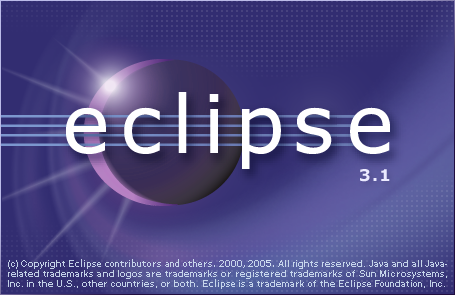
\includegraphics[scale=.5]{image/eclipse-splash}
  \caption{Eclipse}\label{fig:eclipse}
\end{figure}

\subsection{Eclipse Installation}

Eclipse can be downloaded for free from \url{http://www.eclipse.org}.
There you can get a file appropriate for your operating system
containing the software development kit (SDK). For instance
\begin{description}
\item [eclipse-SDK-3.1-win32.zip]\ \\
  for any decent Windows platform.
\item [eclipse-SDK-3.1-linux-gtk.zip]\ \\
  for Linux on Intel x86 with GTK.
\end{description}

Download the appropriate file and unpack it in the installation
directory. A new subdirectory \texttt{eclipse} will be created
containing all files of Eclipse. You are done with the basic
installation. You can start the \texttt{eclipse} executable found in
the just installed directory.

\begin{figure}[h]
  \centering  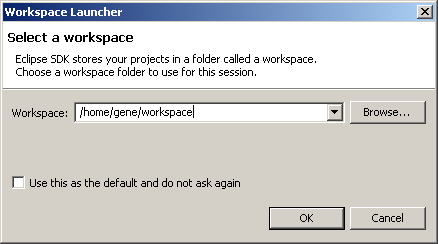
\includegraphics[scale=.5]{image/eclipse-workspace}
  \caption{Eclipse Workspace}\label{fig:eclipse-workspace}
\end{figure}
When Eclipse starts you first see the splash screen shown in
figure~\ref{fig:eclipse}. Then Eclipse requests a workspace -- as
shown in figure~\ref{fig:eclipse-workspace}. The workspace is a
directory where the projects live and where your preferences are
stored. If you have chosen the workspace directory carefully, you can
turn on the check mark in this dialog to be not asked again.

Finally you end up in the welcome window of Eclipse shown in
figure~\ref{fig:eclipse-welcome}. Take some time and read the
introductory material found there.
\begin{figure}[h]
  \centering  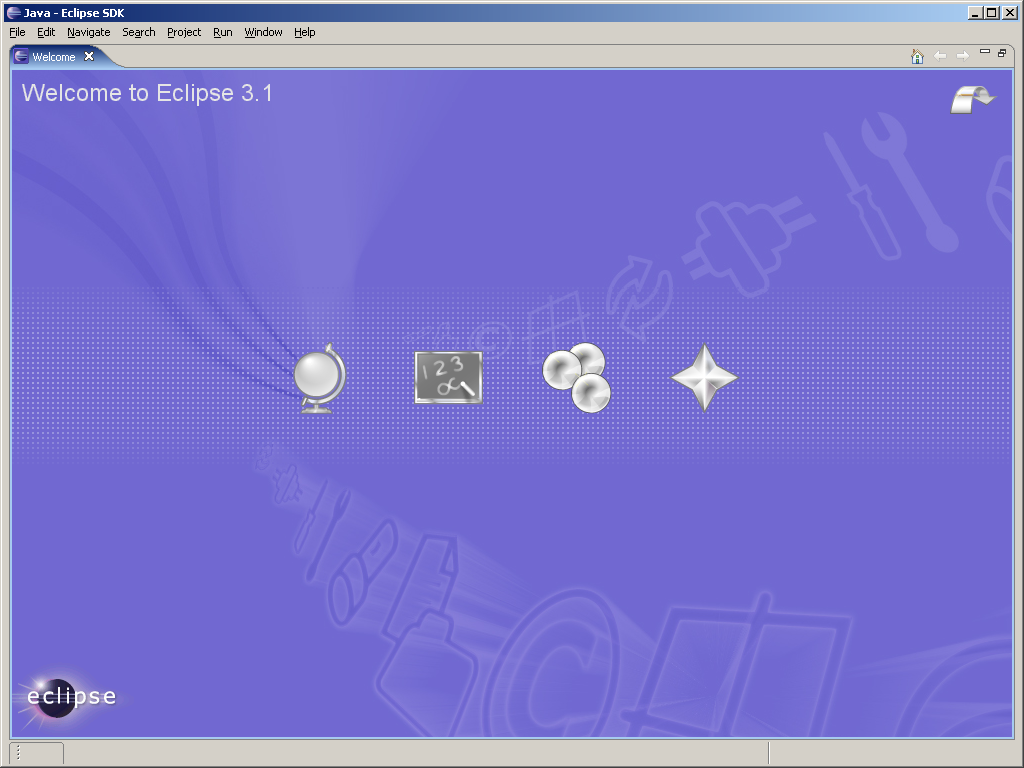
\includegraphics[scale=.25]{image/eclipse-welcome}
  \caption{Eclipse Initial Window}\label{fig:eclipse-welcome}
\end{figure}

The following sections describe some of the configurations which
should be performed in order to work with Eclipse on \ExTeX.


\subsection{Downloading the Sources}

Now we are ready to create a project for the sources of \ExTeX.
Everything needed can be found in the CVs repository of \ExTeX\ hosted
by Berlios.. Thus we start to get things onto the local host. For this
purpose we need to open a new perspective in Eclipse. A perspective is
a collection of windows which are usually meant for a common task.

A new perspective can be opened via the window \menu{Window \sub Open
  Perspective \sub Other\ldots} which can be seen in
figure~\ref{fig:eclipse-open-perspective-menu}.
\begin{figure}[ht]
  \hbox{}\hfill
  \subfigure[Open Perspective\label{fig:A1}]{%
    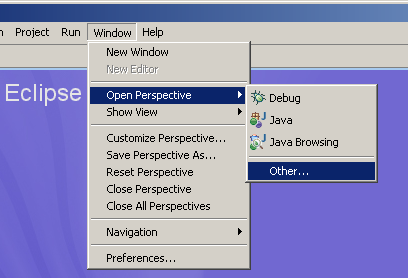
\includegraphics[scale=.4]{image/eclipse-open-perspective-menu}}%
  \hfill
  \subfigure[Selecting ``CVS Exploring Perspective''\label{fig:eclipse-open-perspective-menu}]{%
    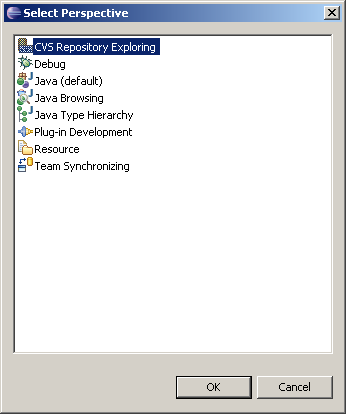
\includegraphics[scale=.4]{image/eclipse-select-cvs}}%
  \hfill\hbox{}

  \caption{Switching to a Perspective}\label{fig:eclipse-perspective}
\end{figure}

This menu item opens a dialog box which offers some perspectives for
opening. Currently we need a ``CVS Exploring'' perspective. This
perspective is meant for inspecting CVS repositories and manipulation.
Thus this perspective is selected (see
figure~\ref{fig:eclipse-select-cvs}) and the dialog is completed with
the OK button.
%\begin{figure}[ht]
%  \centering  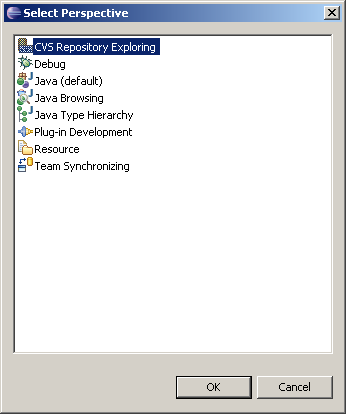
\includegraphics[scale=.4]{image/eclipse-select-cvs}
%  \caption{Selecting ``CVS Exploring Perspective''}\label{fig:eclipse-select-cvs}
%\end{figure}

Now a CVS exploring perspective is opened (see
figure~\ref{fig:eclipse-cvs-1}). You see a lot of windows and icons
there. The tab ``CVS Repositories'' on the left side shows all
repository locations currently known. This list is empty since we have
not added any CVS locations yet.
\begin{figure}[ht]
  \centering  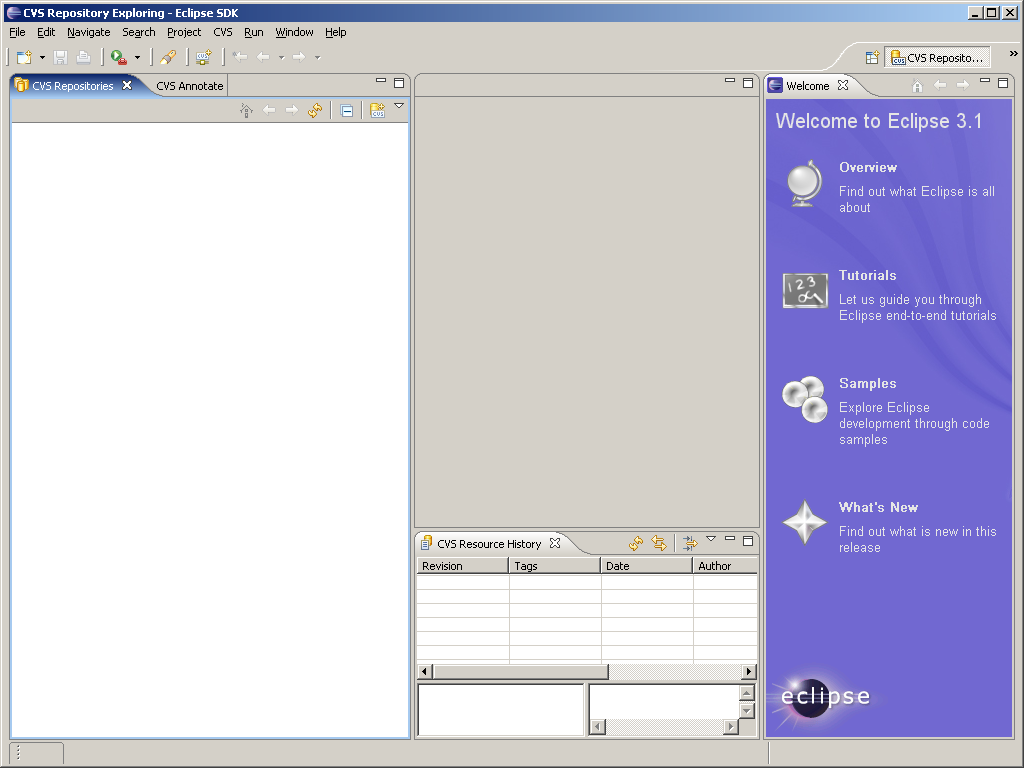
\includegraphics[scale=.25]{image/eclipse-cvs-1}
  \caption{CVS Exploring Perspective}\label{fig:eclipse-cvs-1}
\end{figure}

To add a new repository location press the left mouse button on this
tab and select \menu{New \sub Repository Location\ldots} (see
figure~\ref{fig:eclipse-new-repository}).
\begin{figure}[ht]
  \hbox{}\hfill
  \subfigure[New Repository Location\label{fig:eclipse-new-repository}]{%
    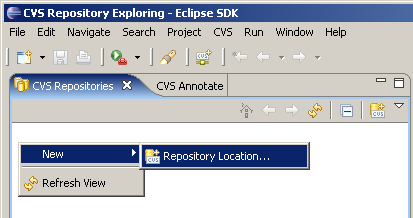
\includegraphics[scale=.4]{image/eclipse-new-repository}}%
  \hfill
  \subfigure[The Coordinates of the \ExTeX\ CVS Repository\label{fig:eclipse-add-cvs}]{%
    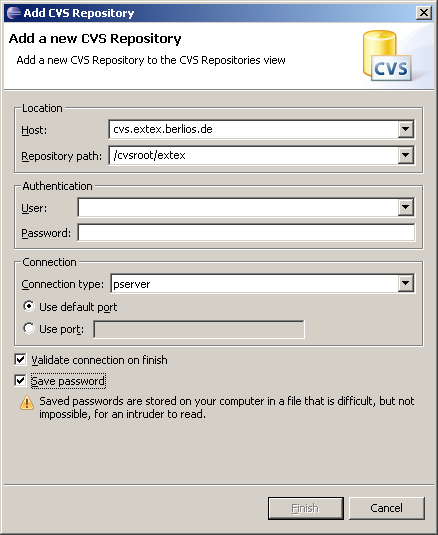
\includegraphics[scale=.4]{image/eclipse-add-cvs}}%
  \caption{Adding the \ExTeX\ CVS Repository}
\end{figure}

This brings up the dialog shown in figure~\ref{fig:eclipse-add-cvs}.
Here you can enter the coordinates of the \ExTeX\ CVS repository.

Note that you have to enter your account at Berlios and its password
into the appropriate fields. If you do not have an account you can use
the account name \texttt{anonymous} without any password to get
reading access to the sources.

For this step you need online access to the internet. When the form is
submitted with the OK button, the accessibility of the repository
location is checked. Upon success the new repository location is
added to the list of repository locations as can be seen in
figure~\ref{fig:eclipse-cvs}.
\begin{figure}[ht]
  \centering  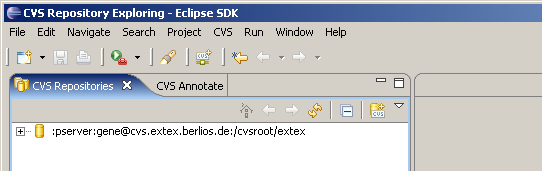
\includegraphics[scale=.4]{image/eclipse-cvs}
  \caption{The \ExTeX\ Repository Listed}\label{fig:eclipse-cvs}
\end{figure}

The next step consists of the check-out of the sources into an Eclipse
project. To accomplish this right-click the repository location in the
list and select \menu{???} in the appearing context menu.

\INCOMPLETE
%\begin{figure}[ht]
%  \centering  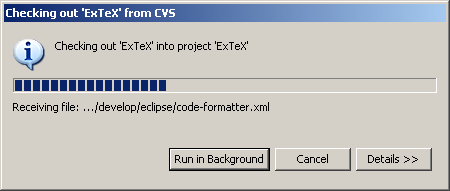
\includegraphics[scale=.4]{image/eclipse-checkout}
%  \caption{The Checkout Progress Bar}\label{fig:eclipse-checkout}
%\end{figure}

\begin{figure}[ht]
  \hbox{}\hfill
  \subfigure[The Checkout Progress Bar\label{fig:eclipse-checkout}]{%
    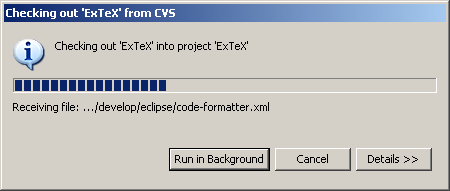
\includegraphics[scale=.4]{image/eclipse-checkout}}%
  \hfill
  \subfigure[The \ExTeX\ Project in the Package View\label{fig:eclipse-extex-project}]{%
    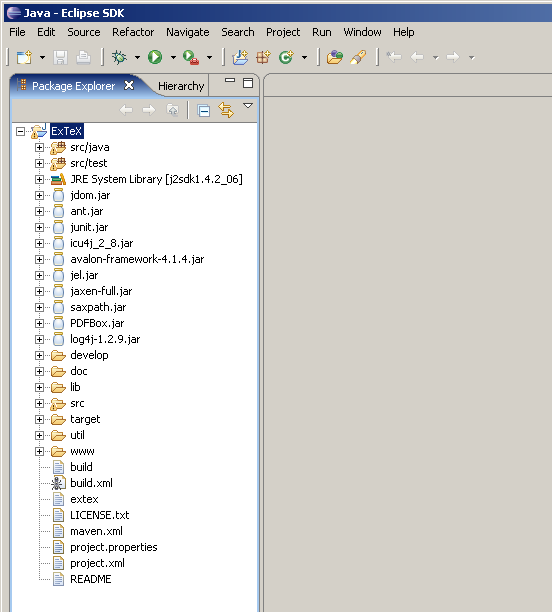
\includegraphics[scale=.4]{image/eclipse-extex-project}}%
  \caption{Checking out \ExTeX\ from the Repository}
\end{figure}

\subsection{Configuring Eclipse}

Eclipse can be configured in a wide range. In the following sections
some configuration options are proposed for the seamless development
of \ExTeX. The configuration is performed via the preferences dialog.
This dialog can be opened via \menu{Window \sub Preferences\ldots}
\begin{figure}[ht]
  \centering  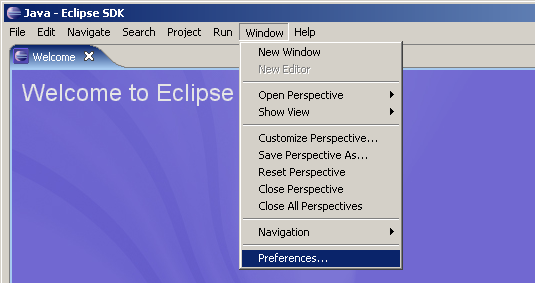
\includegraphics[scale=.4]{image/eclipse-preferences}
  \caption{Eclipse Preferences}\label{fig:eclipse-preferences}
\end{figure}

\begin{figure}[ht]
  \centering  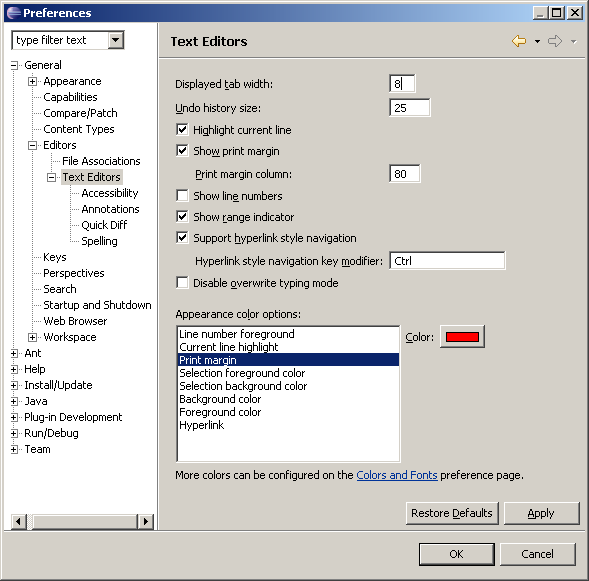
\includegraphics[scale=.4]{image/eclipse-print-margin}
  \caption{Eclipse Print Margin}\label{fig:eclipse-print-margin}
\end{figure}


\subsection{Code Templates}

Code templates provide a convenient way of filling in a frame for the
documentation whenever some code is generated by Eclipse. The \ExTeX\ 
repository contains in the file
\File{develop/eclipse/codetemplates.xml} some definitions of code
templates. To import those definitions use the preferences (see
figure~\ref{fig:eclipse-preferences}). Here select the item \menu{Java
  \sub Code Style \sub Code Templates}. The button \menu{Import\ldots}
can leads to a file selector where the file
\File{develop/eclipse/codetemplates.xml} should be entered.
\begin{figure}[ht]
  \centering  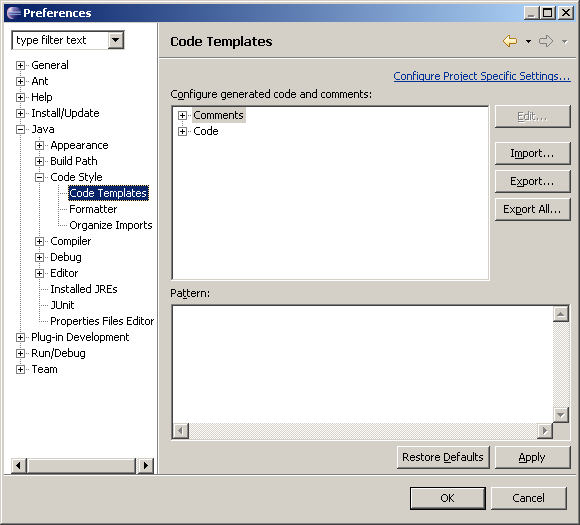
\includegraphics[scale=.4]{image/eclipse-templates}
  \caption{Eclipse Preferences}\label{fig:eclipse-templates}
\end{figure}

After the code templates have been loaded a minor adaption is
required. The entry under the key \menu{Comments \sub Types} containes
hard-wired a name and email address of the author. Here the own name
and email address should be entered.


\subsection{The Code Formatter}

Eclipse comes has a code formatter which can be invoked easily. This
code formatter can be configured for different needs. A configuration
for \ExTeX\ is contained in the repository under
\texttt{develop/eclipse/formatter.xml}.


ant-formatter


\subsection{Checkstyle}

Checkstyle is a tool for checking the adherence of Java source code to
certain rules. The rules can be freely configured. The \ExTeX\
repository contains a set of rules for checkstyle.

Checkstyle comes in a command line version and as a plug-in for
Eclipse. This plugin has to be installed first.

The configuration can be found in \texttt{develop/eclipse/checkstyle-plugin.xml}.


\subsection{Spelling}

Since English is not the native language of each developer it is a
good idea to enable the spell checking of the source code. This
feature is provided by Eclipse. In figure~ref{fig:eclipse-spelling}
you can seen the preference page where you can activate the spell
checking and provide a dictionary.
\begin{figure}[th]
  \centering
  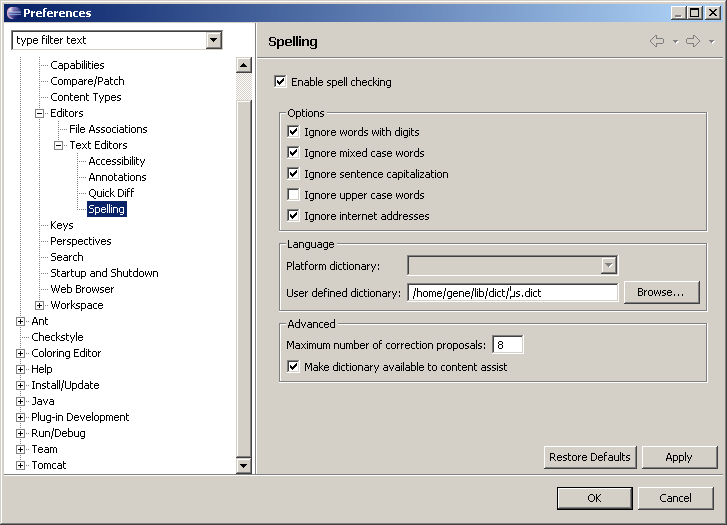
\includegraphics[scale=.4]{image/spelling}
  \caption{Spelling Preferences}\label{fig:eclipse-spelling}
\end{figure}

A dictionary can be got from SCOWL
(\url{http://wordlist.sourceforge.net/}). You might want to use the US
dictionary of medium size. Since this contains enough words to fit but
not too much obscure words which hide typos.

After the spell checking is activated potential typos are marked in
the editor with yellow lines. Correction proposals can be requested
with the quick fix shortcut Ctrl-1.


\subsection{Compiling \ExTeX}

Any source file in Eclipse is compiled automatically when the file is
saved. Thus it is usually not necessary to compile things manually.
If you feel the need to recompile everything you can achieve this by
selecting \menu{Project \sub Clean\ldots} while the item \menu{Project
\sub Build Automatically} is checked (see figure~\ref{fig:eclipse-recompile}).
\begin{figure}[th]
  \centering
  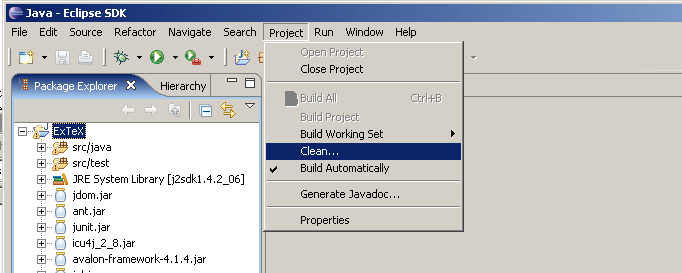
\includegraphics[scale=.4]{image/eclipse-recompile}
  \caption{Recompiling a Project}\label{fig:eclipse-recompile}
\end{figure}

Another recompilation can be triggered via the ant task \texttt{compile}.

\subsection{Running \ExTeX}

\ExTeX\ can be run from within Eclipse.

\INCOMPLETE

\subsection{Committing Changes}

\INCOMPLETE


%------------------------------------------------------------------------------
\section{Command Line Use}
%@author Gerd Neugebauer


\subsection{Downloading the Sources}

You need to download the sources of \ExTeX. On the command line this
can be done with the following commands:

\begin{verbatim}
% cvs -d:pserver:anonymous@cvs.extex.berlios.de:/cvsroot/extex login
% cvs -z3 -d:pserver:anonymous@cvs.extex.berlios.de:/cvsroot/extex co ExTeX
\end{verbatim}


\subsection{Checkstyle}

Checkstyle is a source code checker.
\ExTeX\ should show a homogeneous appearance of the sources.

\INCOMPLETE

\subsection{Ant}

Apache Ant is a build system for Java. It can be considered state of
the art for Java programs to come with ant scripts. \ExTeX\ supports
ant by providing a \texttt{build.xml} file for various tasks.

The files needed for running ant are included in the \ExTeX\
repository. Thus no additional installation is required.


\INCOMPLETE


\subsection{JUnit}

JUnit is the state of the art concerning test automation for Java
programs. Thus \ExTeX\ provides some test cases in the form of JUnit
classes.

\INCOMPLETE


\subsection{Compiling \ExTeX}

Compiling \ExTeX form the command line can be accomplished with the
help of the build script. The build script is a wrapper around Ant. It
can be invoked with the following command:

\begin{verbatim}
  build compile
\end{verbatim}

The generated files are placed in the sub-directory
\texttt{target/classes}. 


\subsection{Running \ExTeX}

\ExTeX\ can be run with the help of the \ExTeX\ script in the main
directory or by a direct invocation of Java. The start script is
provided for Unix under the name \File{extex} and for Windows under
the name \File{extex.bat}.

For the usual purposes these scripts can be used as a plug-in
replacement for \TeX. See the User's Guide for the command line
options.

To run \ExTeX\ from the command line prepare the class path -- i.e.
the environment variable \texttt{CLASSPATH} -- to contain all
libraries found in the directory \texttt{lib}. In addition the
directory \texttt{target/classes} have to be on the class path.
Then you can invoke \ExTeX\ like in the following example:

\begin{verbatim}
  java de.dante.extex.Main.TeX sample.tex
\end{verbatim}

The command line arguments are the same as for \File{extex} mentioned
above.


\subsection{Creating JavaDoc}


\begin{verbatim}
  build javadoc
\end{verbatim}

\INCOMPLETE



\subsection{Creating the Installer}

The installer can be build with the help of the build script. The
invocation looks as follows:

\begin{verbatim}
  build installer
\end{verbatim}

After the work is complete the installer can be found in the file
\texttt{target/ExTeX-setup.jar}. The use of the installer is described
in the User's Manual.

Alternatively the installer can also be created with the Ant task
\texttt{installer}. Using this method can be applied from the command
line and from within Eclipse.

Note that the installer is automatically created once a day and
provided in the snapshot directory of the \ExTeX\ Web site.


%------------------------------------------------------------------------------
\section{Use with Emacs and JDEE}
%@author Gerd Neugebauer

\INCOMPLETE



%------------------------------------------------------------------------------
\section{Modelling: Jude}

Jude is a UML modeller written in Java. It is distributed in a
community edition for free use. Currently the version 1.6.2 is
available from \url{http://www.esm.jp/jude-web/index.html}. 
\begin{figure}[thp]
  \centering
  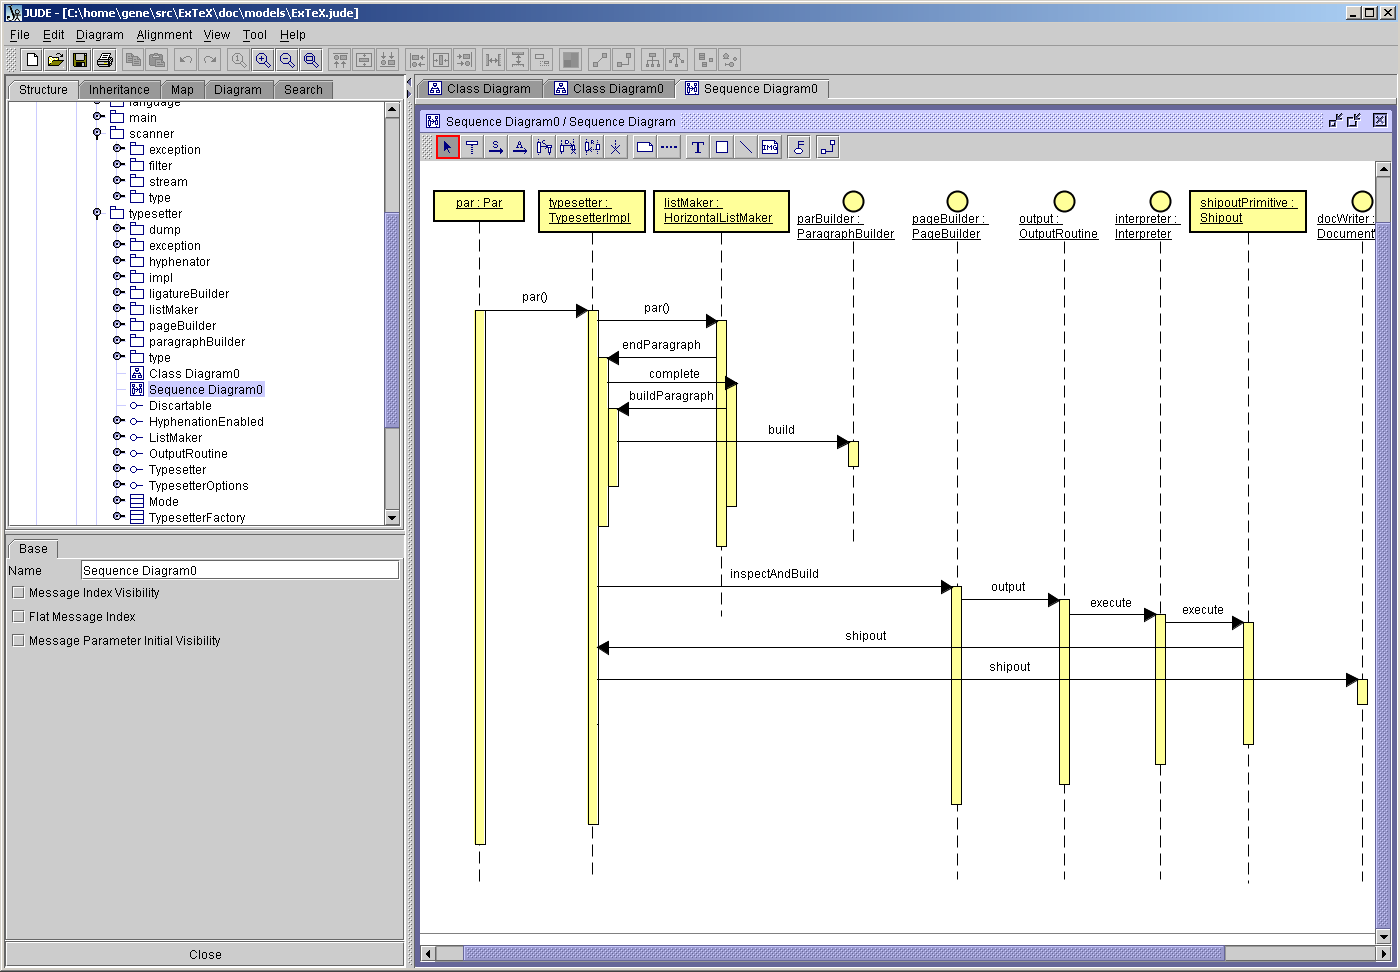
\includegraphics[width=\textwidth]{image/jude-seq}
  \caption{Jude}\label{fig:jude}
\end{figure}

Jude should be used for any situations where UML diagrams are needed.
A screenshot of Jude can be seen in figure~\ref{fig:jude}.

Models for \ExTeX\ should be placed in the directory \File{doc/models}.


%------------------------------------------------------------------------------
\chapter{Source Code Documentation}
%@author Gerd Neugebauer

The source code has to be documented. \TeX\ shows us a good example of
a proper documenatation. Donald Knuth has invented the Web system to
keep together the documentation and the source code. The source code
and documentation are extracted from a common file. In the Java world
the JavaDoc system has been invented for a similar purpose. 

\section{JavaDoc}

The JavaDoc conventions for comments make it possible to extract the
relevant part of the documentation and generate several outut formats
from it. The primary output format is HTML.
\begin{figure}[tbh]
  \centering
  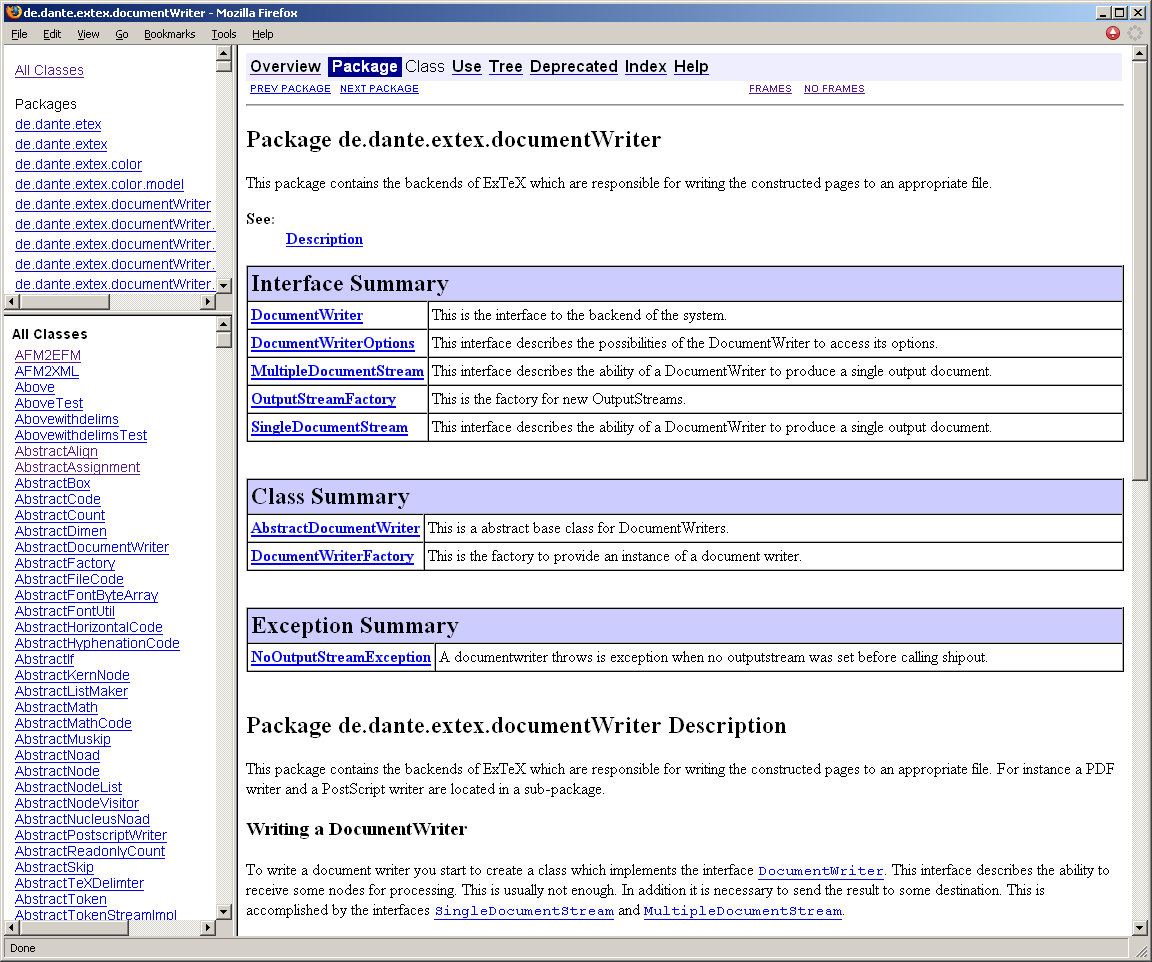
\includegraphics[scale=.25]{image/javadoc}
  \caption{JavaDoc in the Browser}\label{fig:eclipse-javadoc}
\end{figure}

\section{Documentation of Primitives}

\INCOMPLETE




%------------------------------------------------------------------------------
\chapter{The Source Tree Organization}
%@author Gerd Neugebauer

\section{The Toplevel Directory}

The toplevel directory of an \ExTeX\ project contains certain files
and sub-directories.

\begin{description}
\item[develop] \ \\
  The sub-directory \texttt{develop} contains bits and pieces needed
  for development only.
\item[doc]  \ \\
  The sub-directory \texttt{doc} contains documentation -- papers
  written by the \ExTeX\ Group and material collected from elsewhere.
\item[lib]  \ \\
  The sub-directory \texttt{lib} contains libraries which need to be
  present for the final executable to run.
\item[src]  \ \\
  The sub-directory \texttt{src} contains the sources.
\item[target]  \ \\
  The sub-directory \texttt{target} contains the generated files. This
  directory is not present in the CVS archive.
\item[tmp]  \ \\
  The sub-directory \texttt{tmp} may contain intermediary files. This
  directory is not present in the CVS archive.
\item[util]  \ \\
  The sub-directory \texttt{util} contains some utilities for
  development. They are not contained in the installer.
\item[work]  \ \\
  The sub-directory \texttt{work} may contain working files of single
  developers. It is not shared via the repositiory.
\item[www]  \ \\
  The sub-directory \texttt{www} contains the sources for te Web pages
  of \ExTeX.
\end{description}

\section{User's Working Area}

Any user may have some files in the project area, Those files should
not be committed to the Repository. For this purpose the directory
\texttt{work} is reserved.



%------------------------------------------------------------------------------
\chapter{Java Details}
%@author Gerd Neugebauer

\InputIfFileExists{tmp/howto}{}



%------------------------------------------------------------------------------
\chapter{Unit Tests}
%@author Gerd Neugebauer

\INCOMPLETE




%------------------------------------------------------------------------------
\chapter{The Web Pages}
%@author Gerd Neugebauer

\section{Overview}

\ExTeX\ has a domain of its own. This domain \url{www.extex.org} has
been registered by DANTE e.V. In this location the official Web pages
(see figure~\ref{fig:www-eclipse-org}) are provided.
\begin{figure}[htb]
  \centering
  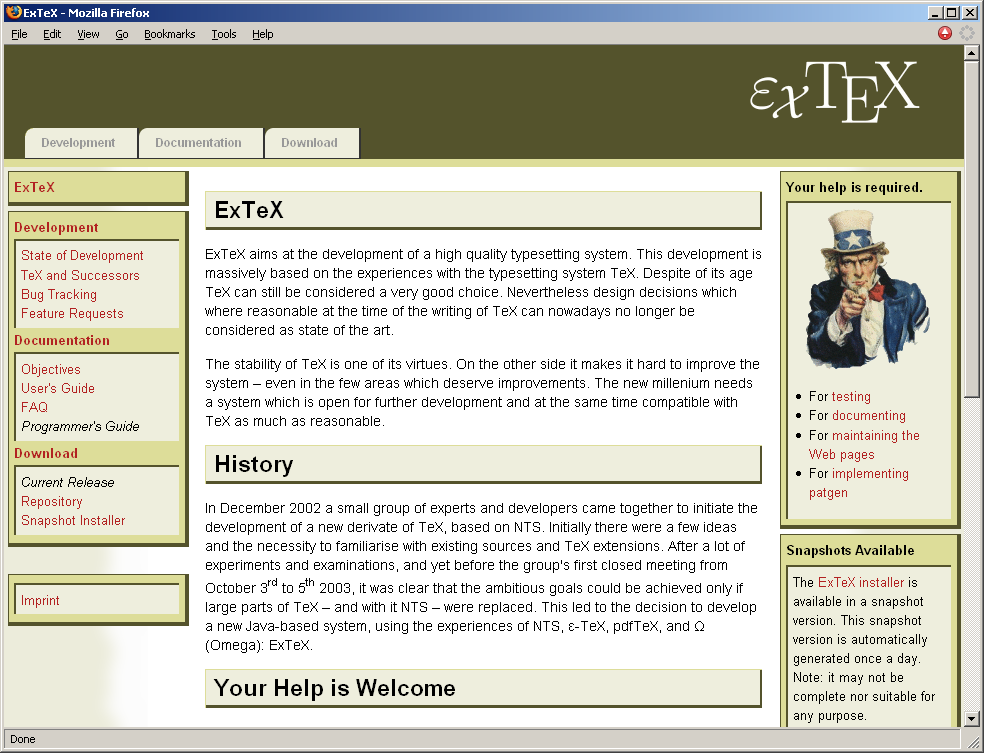
\includegraphics[scale=.4]{image/www-extex-org}
  \caption{www.extex.org}\label{fig:www-extex-org}
\end{figure}

The Web pages are build with a simple generator for a Web site written
in Perl. It has been made for \ExTeX. The aim is the ease of
maintainance for normal content of pages. They are stored as simple
HTML files and augmented automatically upon publication.

The layout is separated form the content and stored in several files.
This makes it very easy to adapt the appearance without touching the
contents.

The sources are kept in the subdirectory \texttt{src}. The generated
files are put into the subdirectory \texttt{www}. Both locations can
be configured.

To generate the Web site run the following command, where the current
directory is the directory \texttt{www}:

\begin{verbatim}
  make
\end{verbatim}

This command creates a complete directory hierarchy with all necessary
sub-directories in \texttt{../target/www}. An exception are the
directories named \texttt{CVS}. Those directories are ignored.

The files starting with \verb|.| or ending in \verb|~| or in
\texttt{.bak} are also ignored. The files not ending in \verb|.html|
are copied into the destination tree. The files ending in \verb|.html|
are processed as follows: Text is inserted before the \verb|</head>|
tag from the file \File{.headEnd}. Text is inserted after the
\verb|<body>| tag from the file \File{.bodyStart}. Text is inserted
before the \verb|</body>| tag from the file \File{.bodyEnd}.

The text to be inserted is sought in the current directory and in case
of failure upwards in the super-directories until it is found. In the
inserted files the following entities and tags are replaced:

\begin{description}
\item [\tt\&top;]\ \\
  this is the relative path to the top directory.
\item [\tt\&year;]\ \\
  this is the current year when generating.
\item [\tt\&month;]\ \\
  this is the current month when generating.
\item [\tt\&day;]\ \\
  this is the current day when generating.
\item [\tt<tabs/>]\ \\
  this is replaced by the contents of the file .tabs.
\item [\tt<navigation/>]\ \\
  this is replaced by the contents of the file .navigation.
\item [\tt<info/>]\ \\
  this is replaced by the contents of the file .info.
\end{description}

Note, that even so it looks like XML processing, currently the
processing is based on string manipulation. Thus tricks possible with
XML might not work here.

\section{Layout}

The current layout has the scheme shown in figure~\ref{fig:www-layout}.
\definecolor{bg}{gray}{.95}
\begin{figure}[htbp]
  \centering

  \definecolor{bg}{gray}{.95}
  \definecolor{shadow}{gray}{.8}
  \begin{pgfpicture}{-1.25mm}{-5mm}{132mm}{51mm}
    
    \begin{pgftranslate}{\pgfpoint{22mm}{41mm}}
      \begin{pgftranslate}{\pgfpoint{1mm}{-1mm}}
        \color{shadow}
        \pgfmoveto{\pgfpoint{0mm}{0mm}} \pgflineto{\pgfpoint{5mm}{10mm}}
        \pgflineto{\pgfpoint{105mm}{10mm}} \pgflineto{\pgfpoint{100mm}{0mm}}
        \pgflineto{\pgfpoint{0mm}{0mm}} \pgffillstroke
      \end{pgftranslate}
      \color{bg}
      \pgfmoveto{\pgfpoint{0mm}{0mm}} \pgflineto{\pgfpoint{5mm}{10mm}}
      \pgflineto{\pgfpoint{105mm}{10mm}} \pgflineto{\pgfpoint{100mm}{0mm}}
      \pgflineto{\pgfpoint{0mm}{0mm}} \pgffillstroke
      \color{black}
      \pgfmoveto{\pgfpoint{0mm}{0mm}} \pgflineto{\pgfpoint{5mm}{10mm}}
      \pgflineto{\pgfpoint{105mm}{10mm}} \pgflineto{\pgfpoint{100mm}{0mm}}
      \pgflineto{\pgfpoint{0mm}{0mm}} \pgfstroke
      \pgfputat{\pgfpoint{52.5mm}{5mm}}{\pgfbox[center,center]{\sf\itshape Header}}
    \end{pgftranslate}
    
    \begin{pgftranslate}{\pgfpoint{18.5mm}{34mm}}
      \begin{pgftranslate}{\pgfpoint{1mm}{-1mm}}
        \color{shadow}
        \pgfmoveto{\pgfpoint{0mm}{0mm}} \pgflineto{\pgfpoint{2.5mm}{5mm}}
        \pgflineto{\pgfpoint{102.5mm}{5mm}} \pgflineto{\pgfpoint{100mm}{0mm}}
        \pgflineto{\pgfpoint{0mm}{0mm}} \pgffillstroke
      \end{pgftranslate}
      \color{bg}
      \pgfmoveto{\pgfpoint{0mm}{0mm}} \pgflineto{\pgfpoint{2.5mm}{5mm}}
      \pgflineto{\pgfpoint{102.5mm}{5mm}} \pgflineto{\pgfpoint{100mm}{0mm}}
      \pgflineto{\pgfpoint{0mm}{0mm}} \pgffillstroke
      \color{black}
      \pgfmoveto{\pgfpoint{0mm}{0mm}} \pgflineto{\pgfpoint{2.5mm}{5mm}}
      \pgflineto{\pgfpoint{102.5mm}{5mm}} \pgflineto{\pgfpoint{100mm}{0mm}}
      \pgflineto{\pgfpoint{0mm}{0mm}} \pgfstroke
      \pgfputat{\pgfpoint{52.5mm}{2.5mm}}{\pgfbox[center,center]{\sf\itshape Tab Bar}}
    \end{pgftranslate}
    
    \begin{pgftranslate}{\pgfpoint{-1mm}{2mm}}
      \begin{pgftranslate}{\pgfpoint{1mm}{-1mm}}
        \color{shadow}
        \pgfmoveto{\pgfpoint{0mm}{0mm}} \pgflineto{\pgfpoint{15mm}{30mm}}
        \pgflineto{\pgfpoint{35mm}{30mm}} \pgflineto{\pgfpoint{20mm}{0mm}}
        \pgflineto{\pgfpoint{0mm}{0mm}} \pgffillstroke
      \end{pgftranslate}
      \color{bg}
      \pgfmoveto{\pgfpoint{0mm}{0mm}} \pgflineto{\pgfpoint{15mm}{30mm}}
      \pgflineto{\pgfpoint{35mm}{30mm}} \pgflineto{\pgfpoint{20mm}{0mm}}
      \pgflineto{\pgfpoint{0mm}{0mm}} \pgffillstroke
      \color{black}
      \pgfmoveto{\pgfpoint{0mm}{0mm}} \pgflineto{\pgfpoint{15mm}{30mm}}
      \pgflineto{\pgfpoint{35mm}{30mm}} \pgflineto{\pgfpoint{20mm}{0mm}}
      \pgflineto{\pgfpoint{0mm}{0mm}} \pgfstroke
      \pgfputat{\pgfpoint{17.75mm}{15mm}}{\pgfbox[center,center]{\parbox{20mm}{\centering\sf\itshape
            Navigation\\Area~~~}}}
    \end{pgftranslate}
    
    \begin{pgftranslate}{\pgfpoint{22mm}{2mm}}
      \begin{pgftranslate}{\pgfpoint{1mm}{-1mm}}
        \color{shadow}
        \pgfmoveto{\pgfpoint{0mm}{0mm}} \pgflineto{\pgfpoint{15mm}{30mm}}
        \pgflineto{\pgfpoint{75mm}{30mm}} \pgflineto{\pgfpoint{60mm}{0mm}}
        \pgflineto{\pgfpoint{0mm}{0mm}} \pgffillstroke
      \end{pgftranslate}
      \color{bg}
      \pgfmoveto{\pgfpoint{0mm}{0mm}} \pgflineto{\pgfpoint{15mm}{30mm}}
      \pgflineto{\pgfpoint{75mm}{30mm}} \pgflineto{\pgfpoint{60mm}{0mm}}
      \pgflineto{\pgfpoint{0mm}{0mm}} \pgffillstroke
      \color{black}
      \pgfmoveto{\pgfpoint{0mm}{0mm}} \pgflineto{\pgfpoint{15mm}{30mm}}
      \pgflineto{\pgfpoint{75mm}{30mm}} \pgflineto{\pgfpoint{60mm}{0mm}}
      \pgflineto{\pgfpoint{0mm}{0mm}} \pgfstroke
      \pgfputat{\pgfpoint{37.5mm}{15mm}}{\pgfbox[center,center]{\sf\itshape
          Content Area}}
    \end{pgftranslate}
    
    \begin{pgftranslate}{\pgfpoint{85mm}{2mm}}
      \begin{pgftranslate}{\pgfpoint{1mm}{-1mm}}
        \color{shadow}
        \pgfmoveto{\pgfpoint{0mm}{0mm}} \pgflineto{\pgfpoint{15mm}{30mm}}
        \pgflineto{\pgfpoint{35mm}{30mm}} \pgflineto{\pgfpoint{20mm}{0mm}}
        \pgflineto{\pgfpoint{0mm}{0mm}} \pgffillstroke
      \end{pgftranslate}
      \color{bg}
      \pgfmoveto{\pgfpoint{0mm}{0mm}} \pgflineto{\pgfpoint{15mm}{30mm}}
      \pgflineto{\pgfpoint{35mm}{30mm}} \pgflineto{\pgfpoint{20mm}{0mm}}
      \pgflineto{\pgfpoint{0mm}{0mm}} \pgffillstroke
      \color{black}
      \pgfmoveto{\pgfpoint{0mm}{0mm}} \pgflineto{\pgfpoint{15mm}{30mm}}
      \pgflineto{\pgfpoint{35mm}{30mm}} \pgflineto{\pgfpoint{20mm}{0mm}}
      \pgflineto{\pgfpoint{0mm}{0mm}} \pgfstroke
      \pgfputat{\pgfpoint{17.5mm}{15mm}}{\pgfbox[center,center]{\parbox{20mm}{\centering\sf\itshape
            Info\\Area~~~}}}
    \end{pgftranslate}
    
    \begin{pgftranslate}{\pgfpoint{-1.25mm}{-5mm}}
      \begin{pgftranslate}{\pgfpoint{1mm}{-1mm}}
        \color{shadow}
        \pgfmoveto{\pgfpoint{0mm}{0mm}} \pgflineto{\pgfpoint{2.5mm}{5mm}}
        \pgflineto{\pgfpoint{102.5mm}{5mm}} \pgflineto{\pgfpoint{100mm}{0mm}}
        \pgflineto{\pgfpoint{0mm}{0mm}} \pgffillstroke
      \end{pgftranslate}
      \color{bg}
      \pgfmoveto{\pgfpoint{0mm}{0mm}} \pgflineto{\pgfpoint{2.5mm}{5mm}}
      \pgflineto{\pgfpoint{102.5mm}{5mm}} \pgflineto{\pgfpoint{100mm}{0mm}}
      \pgflineto{\pgfpoint{0mm}{0mm}} \pgffillstroke
      \color{black}
      \pgfmoveto{\pgfpoint{0mm}{0mm}} \pgflineto{\pgfpoint{2.5mm}{5mm}}
      \pgflineto{\pgfpoint{102.5mm}{5mm}} \pgflineto{\pgfpoint{100mm}{0mm}}
      \pgflineto{\pgfpoint{0mm}{0mm}} \pgfstroke
      \pgfputat{\pgfpoint{52.5mm}{2.5mm}}{\pgfbox[center,center]{\sf\itshape Footer}}
    \end{pgftranslate}
  \end{pgfpicture}

  \caption{Layout of the Web pages}\label{fig:www-layout}
\end{figure}

The Header contains the right aligned Logo only.
It is the same on all pages.
The Tab Bar shows the topmost navigation items with the Tab metophor.
The Navigation Area shows all navigation items.
It is the same on all pages.
The Info Area shows some info items specific for the current
navigation item.

The Content Area contains the contents of the page. This is maintained
by the site authors. The Footer contains a simple copyrigt note.


\section{Automatic Generation}

The web pages are generated automatically every night. This task is
performed with the help of a cron job on shell.berlios.de under the
account gene. In the course of this generation the current sources are
checked out from te CVS repository

Thus the normal user simply has to edit the pages in the area
\texttt{www/src} and check them into the CVS repository. The rest
happens automagically.


%------------------------------------------------------------------------------
\chapter{Licenses for \ExTeX}
%@author Gerd Neugebauer

\INCOMPLETE


%------------------------------------------------------------------------------
\appendix
%------------------------------------------------------------------------------
\chapter{Licenses}
%---------The file header---------------------------------------------
%\documentclass[a4paper,12pt]{book} % possibilities : report book article , etc.
%
%\usepackage[english]{babel} %language selection
%\usepackage[T1]{fontenc}
%
%\pagenumbering{arabic}
%
%\usepackage{hyperref}
%\hypersetup{colorlinks, 
%           citecolor=black,
%           filecolor=black,
%           linkcolor=black,
%           urlcolor=black,
%           pdftex}
%
%           
%\begin{document}
%---------------------------------------------------------------------
\section{GNU Free Documentation License}
\label{label_fdl}

\begin{multicols}{3}\tiny\sf%\scriptsize

 \begin{center}

   Version 1.2, November 2002

   Copyright \copyright\ 2000,2001,2002  Free Software Foundation, Inc.
 
   \bigskip
 
   51 Franklin St, Fifth Floor, Boston, MA  02110-1301  USA
  
   \bigskip
 
   Everyone is permitted to copy and distribute verbatim copies
   of this license document, but changing it is not allowed.
\end{center}


\begin{center}
{\bf Preamble}
\end{center}

The purpose of this License is to make a manual, textbook, or other
functional and useful document ``free'' in the sense of freedom: to
assure everyone the effective freedom to copy and redistribute it,
with or without modifying it, either commercially or noncommercially.
Secondarily, this License preserves for the author and publisher a way
to get credit for their work, while not being considered responsible
for modifications made by others.

This License is a kind of ``copyleft'', which means that derivative
works of the document must themselves be free in the same sense.  It
complements the GNU General Public License, which is a copyleft
license designed for free software.

We have designed this License in order to use it for manuals for free
software, because free software needs free documentation: a free
program should come with manuals providing the same freedoms that the
software does.  But this License is not limited to software manuals;
it can be used for any textual work, regardless of subject matter or
whether it is published as a printed book.  We recommend this License
principally for works whose purpose is instruction or reference.


\begin{center}
{\bf 1. APPLICABILITY AND DEFINITIONS}
%\addcontentsline{toc}{section}{1. APPLICABILITY AND DEFINITIONS}
\end{center}

This License applies to any manual or other work, in any medium, that
contains a notice placed by the copyright holder saying it can be
distributed under the terms of this License.  Such a notice grants a
world-wide, royalty-free license, unlimited in duration, to use that
work under the conditions stated herein.  The \textbf{``Document''}, below,
refers to any such manual or work.  Any member of the public is a
licensee, and is addressed as \textbf{``you''}.  You accept the license if you
copy, modify or distribute the work in a way requiring permission
under copyright law.

A \textbf{``Modified Version''} of the Document means any work containing the
Document or a portion of it, either copied verbatim, or with
modifications and/or translated into another language.

A \textbf{``Secondary Section''} is a named appendix or a front-matter section of
the Document that deals exclusively with the relationship of the
publishers or authors of the Document to the Document's overall subject
(or to related matters) and contains nothing that could fall directly
within that overall subject.  (Thus, if the Document is in part a
textbook of mathematics, a Secondary Section may not explain any
mathematics.)  The relationship could be a matter of historical
connection with the subject or with related matters, or of legal,
commercial, philosophical, ethical or political position regarding
them.

The \textbf{``Invariant Sections''} are certain Secondary Sections whose titles
are designated, as being those of Invariant Sections, in the notice
that says that the Document is released under this License.  If a
section does not fit the above definition of Secondary then it is not
allowed to be designated as Invariant.  The Document may contain zero
Invariant Sections.  If the Document does not identify any Invariant
Sections then there are none.

The \textbf{``Cover Texts''} are certain short passages of text that are listed,
as Front-Cover Texts or Back-Cover Texts, in the notice that says that
the Document is released under this License.  A Front-Cover Text may
be at most 5 words, and a Back-Cover Text may be at most 25 words.

A \textbf{``Transparent''} copy of the Document means a machine-readable copy,
represented in a format whose specification is available to the
general public, that is suitable for revising the document
straightforwardly with generic text editors or (for images composed of
pixels) generic paint programs or (for drawings) some widely available
drawing editor, and that is suitable for input to text formatters or
for automatic translation to a variety of formats suitable for input
to text formatters.  A copy made in an otherwise Transparent file
format whose markup, or absence of markup, has been arranged to thwart
or discourage subsequent modification by readers is not Transparent.
An image format is not Transparent if used for any substantial amount
of text.  A copy that is not ``Transparent'' is called \textbf{``Opaque''}.

Examples of suitable formats for Transparent copies include plain
ASCII without markup, Texinfo input format, \LaTeX\ input format, SGML
or XML using a publicly available DTD, and standard-conforming simple
HTML, PostScript or PDF designed for human modification.  Examples of
transparent image formats include PNG, XCF and JPG.  Opaque formats
include proprietary formats that can be read and edited only by
proprietary word processors, SGML or XML for which the DTD and/or
processing tools are not generally available, and the
machine-generated HTML, PostScript or PDF produced by some word
processors for output purposes only.

The \textbf{``Title Page''} means, for a printed book, the title page itself,
plus such following pages as are needed to hold, legibly, the material
this License requires to appear in the title page.  For works in
formats which do not have any title page as such, ``Title Page'' means
the text near the most prominent appearance of the work's title,
preceding the beginning of the body of the text.

A section \textbf{``Entitled XYZ''} means a named subunit of the Document whose
title either is precisely XYZ or contains XYZ in parentheses following
text that translates XYZ in another language.  (Here XYZ stands for a
specific section name mentioned below, such as \textbf{``Acknowledgements''},
\textbf{``Dedications''}, \textbf{``Endorsements''}, or \textbf{``History''}.)  
To \textbf{``Preserve the Title''}
of such a section when you modify the Document means that it remains a
section ``Entitled XYZ'' according to this definition.

The Document may include Warranty Disclaimers next to the notice which
states that this License applies to the Document.  These Warranty
Disclaimers are considered to be included by reference in this
License, but only as regards disclaiming warranties: any other
implication that these Warranty Disclaimers may have is void and has
no effect on the meaning of this License.


\begin{center}
{\bf 2. VERBATIM COPYING}
%\addcontentsline{toc}{section}{2. VERBATIM COPYING}
\end{center}

You may copy and distribute the Document in any medium, either
commercially or noncommercially, provided that this License, the
copyright notices, and the license notice saying this License applies
to the Document are reproduced in all copies, and that you add no other
conditions whatsoever to those of this License.  You may not use
technical measures to obstruct or control the reading or further
copying of the copies you make or distribute.  However, you may accept
compensation in exchange for copies.  If you distribute a large enough
number of copies you must also follow the conditions in section 3.

You may also lend copies, under the same conditions stated above, and
you may publicly display copies.


\begin{center}
{\bf 3. COPYING IN QUANTITY}
%\addcontentsline{toc}{section}{3. COPYING IN QUANTITY}
\end{center}


If you publish printed copies (or copies in media that commonly have
printed covers) of the Document, numbering more than 100, and the
Document's license notice requires Cover Texts, you must enclose the
copies in covers that carry, clearly and legibly, all these Cover
Texts: Front-Cover Texts on the front cover, and Back-Cover Texts on
the back cover.  Both covers must also clearly and legibly identify
you as the publisher of these copies.  The front cover must present
the full title with all words of the title equally prominent and
visible.  You may add other material on the covers in addition.
Copying with changes limited to the covers, as long as they preserve
the title of the Document and satisfy these conditions, can be treated
as verbatim copying in other respects.

If the required texts for either cover are too voluminous to fit
legibly, you should put the first ones listed (as many as fit
reasonably) on the actual cover, and continue the rest onto adjacent
pages.

If you publish or distribute Opaque copies of the Document numbering
more than 100, you must either include a machine-readable Transparent
copy along with each Opaque copy, or state in or with each Opaque copy
a computer-network location from which the general network-using
public has access to download using public-standard network protocols
a complete Transparent copy of the Document, free of added material.
If you use the latter option, you must take reasonably prudent steps,
when you begin distribution of Opaque copies in quantity, to ensure
that this Transparent copy will remain thus accessible at the stated
location until at least one year after the last time you distribute an
Opaque copy (directly or through your agents or retailers) of that
edition to the public.

It is requested, but not required, that you contact the authors of the
Document well before redistributing any large number of copies, to give
them a chance to provide you with an updated version of the Document.


\begin{center}
{\bf 4. MODIFICATIONS}
%\addcontentsline{toc}{section}{4. MODIFICATIONS}
\end{center}

You may copy and distribute a Modified Version of the Document under
the conditions of sections 2 and 3 above, provided that you release
the Modified Version under precisely this License, with the Modified
Version filling the role of the Document, thus licensing distribution
and modification of the Modified Version to whoever possesses a copy
of it.  In addition, you must do these things in the Modified Version:

\begin{itemize}
\item[A.] 
   Use in the Title Page (and on the covers, if any) a title distinct
   from that of the Document, and from those of previous versions
   (which should, if there were any, be listed in the History section
   of the Document).  You may use the same title as a previous version
   if the original publisher of that version gives permission.
   
\item[B.]
   List on the Title Page, as authors, one or more persons or entities
   responsible for authorship of the modifications in the Modified
   Version, together with at least five of the principal authors of the
   Document (all of its principal authors, if it has fewer than five),
   unless they release you from this requirement.
   
\item[C.]
   State on the Title page the name of the publisher of the
   Modified Version, as the publisher.
   
\item[D.]
   Preserve all the copyright notices of the Document.
   
\item[E.]
   Add an appropriate copyright notice for your modifications
   adjacent to the other copyright notices.
   
\item[F.]
   Include, immediately after the copyright notices, a license notice
   giving the public permission to use the Modified Version under the
   terms of this License, in the form shown in the Addendum below.
   
\item[G.]
   Preserve in that license notice the full lists of Invariant Sections
   and required Cover Texts given in the Document's license notice.
   
\item[H.]
   Include an unaltered copy of this License.
   
\item[I.]
   Preserve the section Entitled ``History'', Preserve its Title, and add
   to it an item stating at least the title, year, new authors, and
   publisher of the Modified Version as given on the Title Page.  If
   there is no section Entitled ``History'' in the Document, create one
   stating the title, year, authors, and publisher of the Document as
   given on its Title Page, then add an item describing the Modified
   Version as stated in the previous sentence.
   
\item[J.]
   Preserve the network location, if any, given in the Document for
   public access to a Transparent copy of the Document, and likewise
   the network locations given in the Document for previous versions
   it was based on.  These may be placed in the ``History'' section.
   You may omit a network location for a work that was published at
   least four years before the Document itself, or if the original
   publisher of the version it refers to gives permission.
   
\item[K.]
   For any section Entitled ``Acknowledgements'' or ``Dedications'',
   Preserve the Title of the section, and preserve in the section all
   the substance and tone of each of the contributor acknowledgements
   and/or dedications given therein.
   
\item[L.]
   Preserve all the Invariant Sections of the Document,
   unaltered in their text and in their titles.  Section numbers
   or the equivalent are not considered part of the section titles.
   
\item[M.]
   Delete any section Entitled ``Endorsements''.  Such a section
   may not be included in the Modified Version.
   
\item[N.]
   Do not retitle any existing section to be Entitled ``Endorsements''
   or to conflict in title with any Invariant Section.
   
\item[O.]
   Preserve any Warranty Disclaimers.
\end{itemize}

If the Modified Version includes new front-matter sections or
appendices that qualify as Secondary Sections and contain no material
copied from the Document, you may at your option designate some or all
of these sections as invariant.  To do this, add their titles to the
list of Invariant Sections in the Modified Version's license notice.
These titles must be distinct from any other section titles.

You may add a section Entitled ``Endorsements'', provided it contains
nothing but endorsements of your Modified Version by various
parties--for example, statements of peer review or that the text has
been approved by an organization as the authoritative definition of a
standard.

You may add a passage of up to five words as a Front-Cover Text, and a
passage of up to 25 words as a Back-Cover Text, to the end of the list
of Cover Texts in the Modified Version.  Only one passage of
Front-Cover Text and one of Back-Cover Text may be added by (or
through arrangements made by) any one entity.  If the Document already
includes a cover text for the same cover, previously added by you or
by arrangement made by the same entity you are acting on behalf of,
you may not add another; but you may replace the old one, on explicit
permission from the previous publisher that added the old one.

The author(s) and publisher(s) of the Document do not by this License
give permission to use their names for publicity for or to assert or
imply endorsement of any Modified Version.


\begin{center}
{\bf 5. COMBINING DOCUMENTS}
%\addcontentsline{toc}{section}{5. COMBINING DOCUMENTS}
\end{center}


You may combine the Document with other documents released under this
License, under the terms defined in section 4 above for modified
versions, provided that you include in the combination all of the
Invariant Sections of all of the original documents, unmodified, and
list them all as Invariant Sections of your combined work in its
license notice, and that you preserve all their Warranty Disclaimers.

The combined work need only contain one copy of this License, and
multiple identical Invariant Sections may be replaced with a single
copy.  If there are multiple Invariant Sections with the same name but
different contents, make the title of each such section unique by
adding at the end of it, in parentheses, the name of the original
author or publisher of that section if known, or else a unique number.
Make the same adjustment to the section titles in the list of
Invariant Sections in the license notice of the combined work.

In the combination, you must combine any sections Entitled ``History''
in the various original documents, forming one section Entitled
``History''; likewise combine any sections Entitled ``Acknowledgements'',
and any sections Entitled ``Dedications''.  You must delete all sections
Entitled ``Endorsements''.

\begin{center}
{\bf 6. COLLECTIONS OF DOCUMENTS}
%\addcontentsline{toc}{section}{6. COLLECTIONS OF DOCUMENTS}
\end{center}

You may make a collection consisting of the Document and other documents
released under this License, and replace the individual copies of this
License in the various documents with a single copy that is included in
the collection, provided that you follow the rules of this License for
verbatim copying of each of the documents in all other respects.

You may extract a single document from such a collection, and distribute
it individually under this License, provided you insert a copy of this
License into the extracted document, and follow this License in all
other respects regarding verbatim copying of that document.


\begin{center}
{\bf 7. AGGREGATION WITH INDEPENDENT WORKS}
%\addcontentsline{toc}{section}{7. AGGREGATION WITH INDEPENDENT WORKS}
\end{center}


A compilation of the Document or its derivatives with other separate
and independent documents or works, in or on a volume of a storage or
distribution medium, is called an ``aggregate'' if the copyright
resulting from the compilation is not used to limit the legal rights
of the compilation's users beyond what the individual works permit.
When the Document is included in an aggregate, this License does not
apply to the other works in the aggregate which are not themselves
derivative works of the Document.

If the Cover Text requirement of section 3 is applicable to these
copies of the Document, then if the Document is less than one half of
the entire aggregate, the Document's Cover Texts may be placed on
covers that bracket the Document within the aggregate, or the
electronic equivalent of covers if the Document is in electronic form.
Otherwise they must appear on printed covers that bracket the whole
aggregate.


\begin{center}
{\bf 8. TRANSLATION}
%\addcontentsline{toc}{section}{8. TRANSLATION}
\end{center}


Translation is considered a kind of modification, so you may
distribute translations of the Document under the terms of section 4.
Replacing Invariant Sections with translations requires special
permission from their copyright holders, but you may include
translations of some or all Invariant Sections in addition to the
original versions of these Invariant Sections.  You may include a
translation of this License, and all the license notices in the
Document, and any Warranty Disclaimers, provided that you also include
the original English version of this License and the original versions
of those notices and disclaimers.  In case of a disagreement between
the translation and the original version of this License or a notice
or disclaimer, the original version will prevail.

If a section in the Document is Entitled ``Acknowledgements'',
``Dedications'', or ``History'', the requirement (section 4) to Preserve
its Title (section 1) will typically require changing the actual
title.


\begin{center}
{\bf 9. TERMINATION}
%\addcontentsline{toc}{section}{9. TERMINATION}
\end{center}


You may not copy, modify, sublicense, or distribute the Document except
as expressly provided for under this License.  Any other attempt to
copy, modify, sublicense or distribute the Document is void, and will
automatically terminate your rights under this License.  However,
parties who have received copies, or rights, from you under this
License will not have their licenses terminated so long as such
parties remain in full compliance.


\begin{center}
{\bf 10. FUTURE REVISIONS OF THIS LICENSE}
%\addcontentsline{toc}{section}{10. FUTURE REVISIONS OF THIS LICENSE}
\end{center}


The Free Software Foundation may publish new, revised versions
of the GNU Free Documentation License from time to time.  Such new
versions will be similar in spirit to the present version, but may
differ in detail to address new problems or concerns.  See
\url{http://www.gnu.org/copyleft/}.

Each version of the License is given a distinguishing version number.
If the Document specifies that a particular numbered version of this
License ``or any later version'' applies to it, you have the option of
following the terms and conditions either of that specified version or
of any later version that has been published (not as a draft) by the
Free Software Foundation.  If the Document does not specify a version
number of this License, you may choose any version ever published (not
as a draft) by the Free Software Foundation.


\begin{center}
{\bf ADDENDUM: How to use this License for your documents}
%\addcontentsline{toc}{section}{ADDENDUM: How to use this License for your documents}
\end{center}

To use this License in a document you have written, include a copy of
the License in the document and put the following copyright and
license notices just after the title page:

%\bigskip
\begin{quote}
    Copyright \copyright  YEAR  YOUR NAME.\\
    Permission is granted to copy, distribute and/or modify this document
    under the terms of the GNU Free Documentation License, Version 1.2
    or any later version published by the Free Software Foundation;
    with no Invariant Sections, no Front-Cover Texts, and no Back-Cover Texts.
    A copy of the license is included in the section entitled ``GNU
    Free Documentation License''.
\end{quote}
%\bigskip
    
If you have Invariant Sections, Front-Cover Texts and Back-Cover Texts,
replace the ``with\dots Texts.'' line with this:

%\bigskip
\begin{quote}
    with the Invariant Sections being LIST THEIR TITLES, with the
    Front-Cover Texts being LIST, and with the Back-Cover Texts being LIST.
\end{quote}
%\bigskip
    
If you have Invariant Sections without Cover Texts, or some other
combination of the three, merge those two alternatives to suit the
situation.

If your document contains nontrivial examples of program code, we
recommend releasing these examples in parallel under your choice of
free software license, such as the GNU General Public License,
to permit their use in free software.

%---------------------------------------------------------------------
%\end{document}
\end{multicols}



\end{document}%%%%%%%%%%%%%%%%%%%%%%%%%%%%%%%%%%%%%%%%%%%%%%%%%%%%%%%%%%%%%%%%%
%
% Local Variables: 
% mode: latex
% TeX-master: nil
% End: 
